\chapter{Metolodología}\label{cap:04metodologia}

A continuación se presentan las metodologías empleadas para desarrollar el proyecto. Para la redacción de la documentación y catálogo de requisitos se ha utilizado el software \ref{sec:04sofia} SofIA y para la planificación temporal se ha utilizado la metodología de gestión de proyectos \ref{sec:04crum} Scrum. El desarrollo completo de la memoria se ha desarrollado mediante \ref{sec:04cvs} Control de versiones.

%Metodología para desarrollar el proyecto
%descripción téorica de los métodos

\section{SofIA} \label{sec:04sofia} %para requisitos

SofIA \cite{escalona2023} es una metodología web dirigida por modelos, cuyo propósito inicial consistió en brindar respaldo a los requisitos del desarrollo web. Fue implementada por primera vez como NDT aunque actualmente ha evolucionado para ofrecer soporte a todo el ciclo de desarrollo, abarcando fases como estudio de viabilidad, requisitos, análisis, diseño, implementación, pruebas y mantenimiento.

Este proyecto se ha beneficiado enormente del uso de SofIA especialmente en la fase de requisitos, que es el núcleo de esta metodología y la razón principal para seguir sus técnicas. Estas facilitarán la captura, definición y validación de una amplia variedad de requisitos.

SofIA no solo ofrece técnicas tradicionales como trazabilidad o prototipos, sino que también aborda otros aspectos como la navegación entre componentes. Esto garantiza una conexión entre todos los elementos y evita inconsistencias en el catálogo de requisitos después de una modificación.

Es importante destacar que SofIA cuenta con un alto grado de automatización y se basa en la herramienta profesional Enterprise Architect \cite{licenciaEA}. En los últimos años, la metodología NDT ha sido ampliamente utilizada como enfoque principal en numerosos proyectos reales de importantes compañías. Entre ellas se destacan entidades públicas como la Consejería de Salud de Andalucía o la Consejería de Cultura de la Junta de Andalucía, así como empresas privadas como Airbus o Everis. 

Esta amplia adopción refleja un alto grado de confianza en la metodología, y se garantiza que su aplicación conducirá al proyecto a desarrollarse en un entorno comparable al de cualquier otro proyecto real, como es el caso de este proyecto.

\section{Scrum} \label{sec:04crum} %para planificación

Scrum \cite{scrumWebsite} consiste en una metodología ágil para la gestión y planificación de proyectos informáticos. En el campo de la informática las metodologías ágiles están en auge, cada vez se opta menos por metodologías tradicionales y se apuesta por estas nuevas metodologías disruptivas. Los motivos y beneficios de ello son muy numerosos, las metodologías ágiles abogan por el cambio continuo y la adaptabilidad frente a la rigurosidad tradicional. 

A continuación se presenta una tabla esquemática de beneficios en el uso de metodologías ágiles.

\begin{table}[H]
\centering
\small % Tamaño del texto reducido
\begin{tabular}{|l|p{5cm}|p{5cm}|} % Reducción del ancho de las columnas
%\begin{tabular}{|l|p{6cm}|p{6cm}|}
\hline
\textbf{Característica} & \textbf{Metodologías Tradicionales} & \textbf{Metodologías Ágiles} \\
\hline
Planificación & Planificación detallada y rígida al inicio del proyecto. & Planificación adaptable y flexible, se adapta a cambios constantes. \\
\hline
Entrega de valor & Entregas al final del proyecto. & Entregas frecuentes de funcionalidades, permitiendo feedback temprano. \\
\hline
%Roles & Roles definidos y fijos. & Equipos multifuncionales con roles flexibles. \\
%\hline
Cambio & Cambios difíciles de gestionar, conllevan retrasos y costos adicionales. & Cambios bienvenidos y gestionados de manera eficiente, se incorporan fácilmente al proyecto. \\
\hline
%Calidad & Pruebas al final del ciclo de desarrollo. & Pruebas continuas e integradas durante todo el proceso. \\
%\hline
Cliente & Interacción limitada con el cliente. & Colaboración estrecha con el cliente, involucrado en todo el proceso. \\
\hline
\end{tabular}
\caption{Comparación de características entre metodologías tradicionales y ágiles en proyectos informáticos.}
\label{tab:metodologias}
\end{table}


Entre las diversas metodologías ágiles, concretamente se ha seleccionado Scrum, que es una solución que se basa en numerosos ciclos iterativos, denominados \textit{sprints}, para el desarrollo incremental del producto final.

\begin{figure}[H]
    \centering
    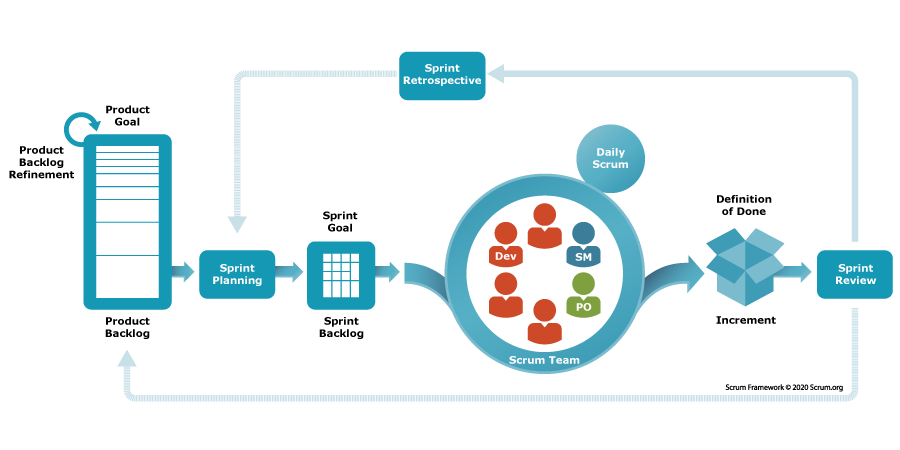
\includegraphics[width=1\textwidth]{figures/scrumFramework.png}
     \caption{Esquema de metodología \textit{Scrum}. Extraída de \cite{scrumWebsite}}
    \label{fig:scrumFramework}
\end{figure}

En la Figura \ref{fig:scrumFramework} ''Esquema de metodología \textit{Scrum}'' se presentan algunos los elementos que intervienen en un proyecto que utiliza la metodología Scrum. A continuación, se identifican los elementos más relevantes de Scrum en este proyecto:

\begin{itemize}
    \item \textbf{\textit{Daily Standup}}: Reuniones diarias para el seguimiento del proyecto, donde se exponen los avances y problemas o dificultades que se han tenido en el transcurso del ciclo diario del proyecto. En el proyecto, esta práctica se llevó a cabo a través de la monitorización continua realizada por los tutores del HUVR.
    \item \textbf{\textit{Product Owner}}: Rol responsable de las características del producto y de asegurar que el equipo aporte valor a la empresa. En el proyecto, este rol es desempeñado por el tutor del HUVR, Carlos Parra (véase \ref{sec:03Participantes} ''Participantes del proyecto'').
    \item \textbf{\textit{Product Backlog}}: Lista priorizada de características que debe tener el producto a desarrollar. En el proyecto, este elemento corresponde al catálogo de requisitos definido conjuntamente con los tutores de la universidad, Julián García y Maria José Escalona (véase \ref{sec:03Participantes} ''Participantes del proyecto'').
    \item \textbf{\textit{Sprint Backlog}}: Conjunto de características escogidas del Product Backlog para implementar en el sprint. En el proyecto, en cada sprint se realizó una división de tareas a realizar, y dentro de cada una se incluyeron un conjunto de subtareas. En esta selección de tareas interviene mayoritariamente la alumna, que es Jefe del Proyecto.
    \item \textbf{\textit{Sprint Review}}: Reunión en la que se presenta y se evalúa el trabajo realizado durante el sprint, con el objetivo de conseguir la aprobación por parte del cliente. En el proyecto, se considera el cliente a los tutores de la universidad, que son los evaluadores del proyecto.
\end{itemize}

El resto de los elementos que aparecen en la Figura \ref{fig:scrumFramework} ''Scrum'' y no se han definido anteriormente, se debe a que no han tenido una aplicación práctica real en el transcurso del proyecto.

\section{Control de versiones} \label{sec:04cvs}

La memoria del trabajo ha sido redactada empleando LaTeX \cite{latex}, un sistema de composición de textos de alta calidad que facilita la creación de documentos estructurados y profesionales, ofreciendo herramientas poderosas fácilemente usables e insertables de manera eficiente.

Para gestionar eficazmente las diferentes versiones del documento, se ha utilizado Github como sistema de control de versiones, subiendo diariamente la última versión del trabajo al repositorio de github del proyecto \cite{vallealonsodc}. GitHub proporciona un entorno seguro donde los cambios realizados por el autor pueden ser registrados, rastreados y revertidos si fuera necesario. Esto garantiza una gestión transparente y organizada del proceso de escritura.

La combinación de LaTeX y GitHub no solo ha facilitado la redacción y edición del Trabajo Fin de Grado, sino que también promueve buenas prácticas en cuanto a la gestión de documentos académicos, asegurando la integridad y trazabilidad de cada versión del mismo.